
\documentclass[11pt]{article}

\usepackage[a4paper,margin=1in]{geometry}
\usepackage{amsmath,amssymb}
\usepackage{bm}
\usepackage{siunitx}
\usepackage{booktabs}
\usepackage{array}
\usepackage[table]{xcolor}
\usepackage{graphicx}
\usepackage{tikz}
\usetikzlibrary{arrows.meta,angles,quotes,calc,positioning}
\usepackage{enumitem}
\usepackage{fancyhdr}
\usepackage[bookmarks,hidelinks]{hyperref}

\definecolor{navy}{HTML}{16324A}
\definecolor{steel}{HTML}{1F4E6B}
\definecolor{rowg}{HTML}{EEF3F7}
\definecolor{cAlpha}{HTML}{1F77B4}
\definecolor{cN}{HTML}{D62728}
\definecolor{cD}{HTML}{2CA02C}
\definecolor{cG}{HTML}{9467BD}
\definecolor{cCom}{HTML}{FF7F0E}

\sisetup{exponent-product=\times}
\DeclareSIUnit{\cm}{cm}
\DeclareSIUnit{\ns}{ns}
\DeclareSIUnit{\MeV}{MeV}
\DeclareSIUnit{\keV}{keV}

\colorlet{headblue}{steel}
\renewcommand{\arraystretch}{1.25}

\newcommand{\code}[1]{\texttt{\small #1}}
\newcommand{\dta}{\mathit{dt}_a}
\newcommand{\dt}{\mathit{dt}}

\pagestyle{fancy}
\fancyhf{}
\renewcommand{\headrulewidth}{0pt}
\renewcommand{\footrulewidth}{0.4pt}
\fancyfoot[L]{\footnotesize\color{gray}API 3D position reconstruction --- derivation \& reconciliation}
\fancyfoot[R]{\footnotesize\color{gray}p.\ \thepage}

\setlength{\parskip}{0.55em}
\setlength{\parindent}{0pt}

\usepackage{titlesec}
\titleformat{\section}{\Large\bfseries\color{navy}}{\thesection.}{0.5em}{}
\titleformat{\subsection}{\large\bfseries\color{steel}}{\thesubsection}{0.5em}{}
\titlespacing*{\section}{0pt}{1.2em}{0.5em}

\begin{document}

\begin{center}
  {\LARGE\bfseries Three-Dimensional Position Reconstruction\\[2pt]
   in the API System}\\[10pt]
  {\large\itshape Mathematical derivation and reconciliation of the
   \code{calcXYZ}, \code{api\_xyz},\\ and thesis (Sec.~4.3) formulations}\\[6pt]
  {\color{gray}\rule{0.6\textwidth}{0.4pt}}
\end{center}

\vspace{0.4em}
\noindent
This note derives, from first principles and for our specific geometry, the
reconstruction of the neutron-interaction point $(x,y,z)$ in the
Associated-Particle Imaging (API) system. The full model (relativistic speeds,
center-of-mass correction, exact gamma-detector vector) is taken as
authoritative; the two simplified implementations and the thesis derivation are
recovered as special cases, and every discrepancy among the three sources is
catalogued in the errata of Section~8.

\section{The reconstruction problem}
In coincidence mode the DAQ reports, per event, the four corner energies of the
YAP alpha detector, the gamma-ray energy, and the alpha--gamma time difference
$\dt$ (Table 4.2 of the thesis). Reconstruction proceeds in four steps:
\begin{itemize}[leftmargin=1.4em,itemsep=2pt]
  \item \textbf{Step A --- Alpha position.} The four corner energies give the
        alpha interaction point $(x_0,y_0)$ on the YAP face (Section~3).
  \item \textbf{Step B --- Neutron direction and speed.} Momentum conservation
        in the D--T reaction fixes the neutron velocity vector from the alpha
        direction, including the center-of-mass motion (Section~4).
  \item \textbf{Step C --- Time of flight.} The measured $\dt$, the alpha flight
        time $t_\alpha$, and the gamma flight time tie the neutron path length to
        the geometry (Section~5).
  \item \textbf{Step D --- Solve for the point.} A single quadratic in the
        neutron flight time yields $(x,y,z)$ (Section~6).
\end{itemize}
The tagged neutron travels essentially opposite to the detected alpha, so the
alpha hit defines a \emph{ray} from the source into the sample; the timing fixes
\emph{how far} along that ray the gamma-producing scatter occurred.

\section{Coordinate system and geometry}
We place the origin $O$ at the neutron production point (the reaction spot inside
the generator head) and let the $+z$ axis point along the API cone axis, into the
sample volume. This is the choice made by \code{calcXYZ}; it is the cleanest
because the neutron starts at the origin, so both the interaction point and the
gamma detector are referred to the same point. The YAP alpha-detector face lies
at $z=-z_t$, and the alpha interacts at $A=(x_0,y_0,-z_t)$.

\begin{center}
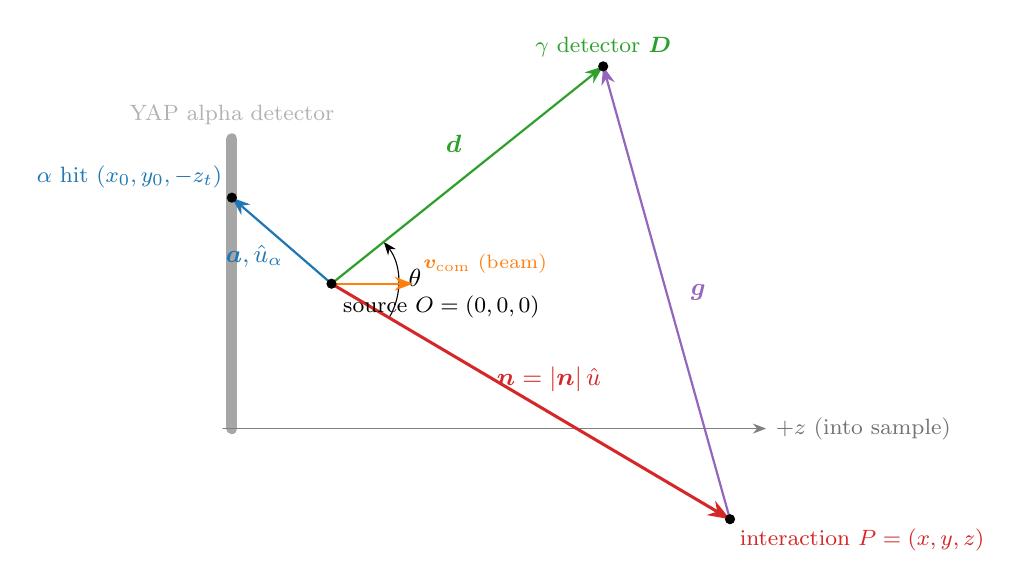
\begin{tikzpicture}[>=Stealth,scale=1.15,
   vec/.style={thick,->},line cap=round]
  \coordinate (O) at (0,0);
  \coordinate (A) at (-1.1,0.95);
  \coordinate (P) at (4.4,-2.6);
  \coordinate (D) at (3.0,2.4);
  % YAP crystal face
  \draw[line width=4pt,gray!70] (-1.1,-1.6) -- (-1.1,1.6);
  \node[gray!60,above,font=\footnotesize] at (-1.1,1.65) {YAP alpha detector};
  % z axis
  \draw[->,gray,thin] (-1.2,-1.6) -- (4.8,-1.6)
       node[right,font=\footnotesize,black!55] {$+z$ (into sample)};
  % angle
  \pic[draw,->,"\small$\theta$",angle radius=0.85cm,angle eccentricity=1.25]
       {angle=P--O--D};
  % vectors
  \draw[vec,cCom] (O) -- (0.9,0) node[above right,font=\scriptsize,cCom]
       {$\bm{v}_{\mathrm{com}}$ (beam)};
  \draw[vec,cAlpha] (O) -- (A);
  \draw[vec,cN,line width=1.1pt] (O) -- (P);
  \draw[vec,cD] (O) -- (D);
  \draw[vec,cG] (P) -- (D);
  % points
  \foreach \p in {O,A,P,D}{\fill (\p) circle (1.6pt);}
  % labels
  \node[cAlpha,above left,font=\footnotesize] at (A) {$\alpha$ hit $(x_0,y_0,-z_t)$};
  \node[cD,above,font=\footnotesize] at (D) {$\gamma$ detector $\bm{D}$};
  \node[cN,below right,font=\footnotesize] at (P) {interaction $P=(x,y,z)$};
  \node[below right=1pt,font=\footnotesize] at (O) {source $O=(0,0,0)$};
  \node[cAlpha,font=\small] at (-0.85,0.30) {$\bm{a},\hat u_\alpha$};
  \node[cN,font=\small] at (2.4,-1.05) {$\bm{n}=|\bm{n}|\,\hat u$};
  \node[cD,font=\small] at (1.35,1.55) {$\bm{d}$};
  \node[cG,font=\small] at (4.05,-0.1) {$\bm{g}$};
\end{tikzpicture}
\end{center}
{\footnotesize\color{black!60}\textbf{Figure 1.} Reconstruction geometry
(projected on the $y$--$z$ plane). The alpha hit on the YAP defines the ray
direction; the timing fixes the neutron path length $|\bm{n}|$. Vectors
$\bm a,\bm n,\bm d,\bm g$ and the angle $\theta$ are used in the derivation.}

\vspace{0.6em}
Our specific geometry uses the following fixed quantities:

\begin{center}
\begin{tabular}{>{\raggedright}p{1.6cm} p{6.4cm} p{6.0cm}}
\toprule
\rowcolor{steel}\color{white}\textbf{Symbol} & \color{white}\textbf{Meaning} & \color{white}\textbf{Value (this system)}\\
$z_t$ & source $\rightarrow$ YAP-face distance & \SI{6.7}{\cm}\\
\rowcolor{rowg}$a$ & YAP active square side & \SI{4.8}{\cm} ($\pm\SI{2.4}{\cm}$)\\
$v_\alpha$ & alpha speed (\SI{3.5}{\MeV}, relativistic) & \SI{1.298e+07}{\meter\per\second} ($\beta=0.0433$)\\
\rowcolor{rowg}$v_n$ & neutron speed (\SI{14.1}{\MeV}, relativistic) & \SI{5.136e+07}{\meter\per\second} ($\beta=0.1713$)\\
$v_{\mathrm{com}}$ & center-of-mass speed (\SI{50}{\keV} $\mathrm{D}^+$) & \SI{8.764e+05}{\meter\per\second} ($\beta=0.00292$)\\
\rowcolor{rowg}$c$ & speed of light $=v_\gamma$ & \SI{2.997925e+08}{\meter\per\second}\\
$\hat C$ & ion-beam unit vector ($v_{\mathrm{com}}$ dir.) & \code{meta['ion beam axis']}\\
\rowcolor{rowg}$\bm D$ & gamma-detector centre & \code{meta['detectors'][k]['position']}\\
\bottomrule
\end{tabular}
\end{center}

In \code{calcXYZ} the symbol \code{meta['scintillator distance']} \emph{is} $z_t$:
it is the $z$ of the alpha hit, \code{Z\_alpha = scintillator\_dz}. The thesis
quotes $z_t=\SI{6}{\cm}$ in the text; the code uses \SI{6.7}{\cm}, which we adopt
here (see errata, Section~8).

\section{Step A --- alpha position from the four corners}
The YAP is read out at its four corners $A,B,C,D$ (charge division). Labelling
them so that $B$ is the $+x,+y$ corner, $A$ the $-x,+y$, $C$ the $+x,-y$, and $D$
the $-x,-y$ corner, the normalised coordinates are
\begin{equation}
  x_{\mathrm{raw}}=\frac{B+C-D-A}{A+B+C+D},\qquad
  y_{\mathrm{raw}}=\kappa\,\frac{B+A-D-C}{A+B+C+D},
\end{equation}
where $\kappa=1.305$ is an empirical factor that makes the measured alpha image
square (\code{map\_alpha\_XY}). Note \code{calc\_own\_pos} / the \code{X2,Y2}
columns used by the GUI omit $\kappa$ (set it to $1$) and apply the squaring later
through edge detection --- numerically equivalent once the axis is scaled to
centimetres.

The dimensionless values are mapped to physical centimetres across the
\SI{4.8}{\cm} active face. Rather than trust the absolute gain, the code locates
the populated edges of the alpha image (the histogram region above ${\sim}1/3$ of
the peak) and linearly maps that span onto $[-2.4,+2.4]\,\si{\cm}$:
\begin{equation}
  x_0=\frac{a}{x_{\max}-x_{\min}}\,(x_{\mathrm{raw}}-x_{\max})+\frac{a}{2},
  \qquad a=\SI{4.8}{\cm},
\end{equation}
and similarly for $y_0$. (The legacy \code{map\_alpha\_XY} additionally flips the
$x$-axis so an $X$--$Y$ image matches the view from in front of the experiment,
and can apply spline edge-corrections from the \code{DX/DY} lookup tables.) The
output of Step~A is the alpha interaction point $(x_0,y_0)$ in centimetres on the
YAP face.

\section{Step B --- neutron velocity vector}

\subsection{Naive (back-to-back) direction}
If the neutron and alpha left the source exactly \ang{180} apart, the neutron
direction is simply opposite the source$\rightarrow$alpha vector. With the alpha
hit at $A=(x_0,y_0,-z_t)$,
\begin{equation}
  \bm a=\langle x_0,\,y_0,\,-z_t\rangle,\qquad
  \hat u=-\frac{\bm a}{|\bm a|}
        =\frac{\langle -x_0,\,-y_0,\,z_t\rangle}{\sqrt{x_0^2+y_0^2+z_t^2}}.
\end{equation}
This is exactly the thesis vector (eq.~4.5) and what \code{api\_xyz} uses
($u_x=-x_a/|\bm a|$, $u_z=+z_a/|\bm a|$ with $z_a=\SI{6.7}{\cm}$). The thesis
takes the origin at the YAP centre rather than the source, but the
\emph{direction} $\hat u$ is identical.

\subsection{Center-of-mass correction (the full model)}
The \ang{180} assumption holds only in the reaction center-of-mass (CM) frame.
The $\mathrm{{}^2H}+\mathrm{{}^3H}\rightarrow\mathrm{{}^4He}+n$ reaction is driven
by a deuteron beam, so the CM moves in the lab with a small velocity along the
beam axis $\hat C$:
\begin{equation}
  \bm v_{\mathrm{com}}=v_{\mathrm{com}}\,\hat C,\qquad
  v_{\mathrm{com}}=\frac{\sqrt{2\,m_d E_d}}{m_d+m_t}\,c\approx 0.00292\,c .
\end{equation}
For a \SI{50}{\keV} deuteron beam this is
$v_{\mathrm{com}}\approx\SI{8.764e+05}{\meter\per\second}$. Although tiny
($\beta_{\mathrm{com}}\approx0.00292$), it tilts the lab neutron direction away
from exact \ang{180} by up to ${\approx}\ang{0.98}$, i.e.\ roughly
\SI{1.2}{\cm} of transverse displacement at a \SI{70}{\cm} stand-off ---
comparable to the system resolution and therefore worth correcting.
\code{calcXYZ} reads $v_{\mathrm{com}}$ versus beam energy from
\code{center-of-mass.npy}; the formula above reproduces it from the reaction
kinematics.

The construction has three parts. First the alpha flight time $t_\alpha$ is found
by requiring that, in the CM frame, the alpha travels at speed $v_\alpha$:
\begin{equation}
  |\bm A-\bm v_{\mathrm{com}}\,t_\alpha|=v_\alpha\,t_\alpha
  \ \Longrightarrow\
  (v_\alpha^2-v_{\mathrm{com}}^2)\,t_\alpha^2
   +2(\bm A\cdot\bm v_{\mathrm{com}})\,t_\alpha-|\bm A|^2=0,
\end{equation}
taking the positive root. The alpha velocity in the CM frame is then
$\bm w_\alpha=(\bm A-\bm v_{\mathrm{com}}t_\alpha)/t_\alpha$, and because the
neutron is exactly opposite the alpha \emph{in the CM frame}, the neutron
velocity in the lab is
\begin{equation}
  \bm v_n=-\frac{\bm w_\alpha}{v_\alpha}\,v_n+\bm v_{\mathrm{com}},
\end{equation}
i.e.\ (neutron CM direction)$\times$(neutron CM speed)$+$(CM drift). This is
exactly the two-line update in \code{calcXYZ}
(\code{vn\_x = -vn\_x/v\_alpha*v\_neutron + v\_com\_vector[0]}, \ldots). In the
naive model $v_{\mathrm{com}}\to0$ and $\bm v_n=v_n\hat u$.

\section{Step C --- the time-of-flight relation}
The recorded $\dt$ is the alpha--gamma time difference. Writing $t_n,t_g,t_\alpha$
for the neutron, gamma, and alpha flight times, the thesis relation (eq.~4.7) is
\begin{equation}
  \dt=t_n+t_g-t_\alpha
  \quad\Longrightarrow\quad
  \dta\equiv \dt+t_\alpha=t_n+t_g,
\end{equation}
so folding the alpha flight time into the time difference defines a single
quantity $\dta$. (Per-detector electronic offsets --- the \code{z-align}
constants and the ${\approx}\SI{11}{\ns}$ PMT transit delay noted in the thesis
--- are subtracted from $\dt$ before this step; they shift the zero of $\dt$ but
do not change the algebra below.) In \code{calcXYZ} this is literally
\code{df['dt'] = dt\_orig + t\_alpha} followed by the channel-wise offset
subtraction.

\section{Step D --- solving for the interaction point}
Let $\bm D$ be the gamma-detector centre and $\bm P=\bm v_n t_n$ the interaction
point (the neutron starts at the origin with lab velocity $\bm v_n$). The gamma
then travels from $\bm P$ to $\bm D$ at speed $c$ in the remaining time
$t_g=\dta-t_n$:
\begin{equation}
  |\bm D-\bm v_n\,t_n|^2=c^2\,(\dta-t_n)^2 .
\end{equation}
Expanding gives a quadratic in the neutron flight time,
$\alpha' t_n^2+\beta' t_n+\gamma'=0$, with
\begin{equation}
  \alpha'=c^2-|\bm v_n|^2,\qquad
  \beta'=-\bigl(2c^2\dta-2\,\bm D\cdot\bm v_n\bigr),\qquad
  \gamma'=c^2\dta^2-|\bm D|^2 .
\end{equation}
Our coordinate choice selects the negative root:
\begin{equation}
  t_n=\frac{-\beta'-\sqrt{\beta'^2-4\alpha'\gamma'}}{2\alpha'},
  \qquad (x,y,z)=\bm v_n\,t_n .
\end{equation}
This is exactly the second quadratic in \code{calcXYZ} (coefficients
\code{a,b,c} and \code{t\_neutron}); the reconstructed point is
\code{X=vn\_x*t\_neutron}, etc. It uses the \emph{exact} detector vector
$\bm D-\bm P$; no point-source or law-of-cosines approximation enters.

\subsection{The thesis / \texorpdfstring{\code{api\_xyz}}{api\_xyz} special case}
If we drop the CM correction (so $|\bm v_n|=v_n$ and $\bm v_n=v_n\hat u$) and
solve instead for the path length $|\bm n|=v_n t_n$, the gamma constraint becomes
the law of cosines (thesis eq.~4.8)
\begin{equation}
  |\bm g|^2=|\bm d|^2+|\bm n|^2-2|\bm d|\,|\bm n|\cos\theta,\qquad
  \cos\theta=\frac{u_x x_1+u_y y_1+u_z z_1}{|\bm d|},
\end{equation}
which, combined with $|\bm g|=c(\dta-|\bm n|/v_n)$, yields the thesis quadratic
(eqs.~4.9--4.10)
\begin{equation}
  a=1-\frac{c^2}{v_n^2},\qquad
  b=\frac{2\dta c^2}{v_n}-2|\bm d|\cos\theta,\qquad
  c=|\bm d|^2-c^2\dta^2,
\end{equation}
\begin{equation}
  |\bm n|=\frac{-b-\sqrt{b^2-4ac}}{2a},\qquad
  x=\frac{-x_0}{|\bm a|}|\bm n|,\quad
  y=\frac{-y_0}{|\bm a|}|\bm n|,\quad
  z=\frac{z_t}{|\bm a|}|\bm n|+z_t .
\end{equation}
This is precisely \code{api\_xyz(use\_det=True)}. The two forms agree when
$v_{\mathrm{com}}\to0$ \emph{and} when $\bm d$ is measured from the same point as
$\bm n$ --- which exposes the origin inconsistency discussed in the errata.
Setting \code{use\_det=False} drops the detector term entirely, leaving the
straight-ray estimate $|\bm n|=v_n\dta$; this is the crudest variant and is, at
present, the one the wara GUI uses.

\clearpage
\section{Reconciliation of the three implementations}
All three sources implement the same idea at increasing levels of rigour.

\begin{center}
\begin{tabular}{p{3.0cm} p{2.9cm} p{2.9cm} p{3.0cm}}
\toprule
\rowcolor{steel}\color{white}\textbf{Aspect} & \color{white}\textbf{Thesis Sec.\ 4.3} & \color{white}\textbf{\code{api\_xyz} (-{}-beta)} & \color{white}\textbf{\code{calcXYZ}}\\
Coordinate origin & YAP centre & YAP centre & neutron source\\
\rowcolor{rowg}Source--YAP $z_t$ & \SI{6}{\cm} & \SI{6.7}{\cm} & meta scint.\ dist.\\
Particle speeds & symbolic & non-relativistic & relativistic\\
\rowcolor{rowg}$\alpha$--$n$ back-to-back & exact \ang{180} & exact \ang{180} & CM-corrected\\
Gamma detector & law of cosines & cosines / ignored & exact $\bm D-\bm P$\\
\rowcolor{rowg}Units & --- & cm, $c=\num{3e10}$ & SI, scipy $c$\\
Solves for & $|\bm n|$ (path) & $|\bm n|$ (path) & $t_n$ (then $\bm v_n t_n$)\\
\rowcolor{rowg}Quadratic root & negative & negative & negative\\
\bottomrule
\end{tabular}
\end{center}

\section{Errata and resolved discrepancies}
The following issues were found while reconciling the three sources. Items 1--4
are genuine physics/algebra points; items 5--6 are bookkeeping.
\begin{enumerate}[leftmargin=1.5em,itemsep=4pt]
  \item \textbf{Thesis typo (minor).} The constant term of eq.~4.10 is printed as
        $c=|\bm d|^2-c^2\dt^2$ but should use $\dta$, i.e.\
        $c=|\bm d|^2-c^2\dta^2$. (The stray subscript ``$a$'' is dropped to the
        next line in the PDF.) The rest of the derivation is self-consistent.
  \item \textbf{Law-of-cosines origin mismatch (thesis \& \code{api\_xyz}).} The
        neutron path $\bm n$ is measured from the source at $(0,0,z_t)$, but
        $\bm d$ and $\cos\theta$ are measured from the YAP centre. The law of
        cosines treats them as sharing one vertex, so the gamma path length is
        off by ${\sim}z_t$ in $z$. Putting the origin at the source (full model)
        removes this: $\bm D$ and $\bm P$ share the origin and
        $|\bm g|=|\bm D-\bm P|$ is exact.
  \item \textbf{Non-relativistic speeds (\code{api\_xyz}).} Using $\sqrt{2E/m}$
        overestimates the neutron speed: $\beta_n=0.1732$ vs $0.1713$
        relativistic, ${\sim}1.1\%$ high. Over a ${\sim}\SI{70}{\cm}$ flight
        this biases $Z$ at the centimetre scale. The full model uses the
        relativistic $\beta$.
  \item \textbf{\ang{180} back-to-back assumption (thesis \& \code{api\_xyz}).}
        Ignores the lab-frame CM momentum; the neutron is back-to-back with the
        alpha only in the CM frame. This tilts the ray by up to
        ${\sim}\ang{0.98}$ (${\sim}\SI{1.2}{\cm}$ at \SI{70}{\cm}).
        The full model corrects it via $\bm v_{\mathrm{com}}$ --- precisely the
        dominant error source the thesis itself flags.
  \item \textbf{$z_t$ value.} \SI{6}{\cm} (thesis text) vs \SI{6.7}{\cm} (code).
        We adopt \SI{6.7}{\cm}, matching \code{api\_xyz}, \code{helper\_api}, and
        the as-built code.
  \item \textbf{Sign / origin convention.} \code{api\_xyz} puts the sample at
        $+z$ with the YAP centre as origin; \code{calcXYZ} puts the origin at the
        source. They are related by a translation of $z_t$ along $z$ (and a sign
        flip of the $z$-axis). Reconstructed depths must be interpreted in the
        convention of whichever routine produced them.
\end{enumerate}

\noindent\textbf{Practical consequence for the GUI.} The GUI currently calls
\code{api\_xyz(use\_det=False)}, the crudest path (non-relativistic, no CM
correction, detector ignored). Migrating the GUI to the full \code{calcXYZ} model
--- or at minimum enabling the detector term and relativistic speeds --- is the
natural follow-up to this note.

\clearpage
\section{Worked numerical example}
To make the formulas checkable, we reconstruct one synthetic event with the full
model. Inputs (origin at source, $+z$ into the sample):
\begin{itemize}[leftmargin=1.4em,itemsep=2pt]
  \item alpha hit on the YAP: $(x_0,y_0)=(1.20,-0.80)\,\si{\cm}$, at
        $z=-\SI{6.7}{\cm}$;
  \item measured time difference: $\dt=\SI{18.0}{\ns}$;
  \item beam axis $\hat C=(0,0,1)$; $v_{\mathrm{com}}=\SI{8.764e+05}{\meter\per\second}$;
  \item illustrative gamma-detector centre:
        $\bm D=(0,30,35)\,\si{\cm}$.
\end{itemize}
Intermediate and final results:

\begin{center}
\begin{tabular}{p{8.2cm} p{5.0cm}}
\toprule
\rowcolor{steel}\color{white}\textbf{Quantity} & \color{white}\textbf{Value}\\
alpha flight time $t_\alpha$ & \SI{5.653}{\ns}\\
\rowcolor{rowg}$\dta=\dt+t_\alpha$ & \SI{23.653}{\ns}\\
neutron flight time $t_n$ (full) & \SI{21.075}{\ns}\\
\rowcolor{rowg}$\bm P$, full model (det $+$ CM $+$ rel.) & $(-17.70,\ 11.80,\ 107.98)\,\si{\cm}$\\
$\bm P$, detector ignored (-{}-beta path) & $(-19.54,\ 13.03,\ 119.19)\,\si{\cm}$\\
\rowcolor{rowg}$\bm P$, thesis (non-rel, no CM) & $(-18.89,\ 12.59,\ 105.47)\,\si{\cm}$\\
depth difference full $-$ thesis ($z$) & \SI{+2.51}{\cm}\\
\bottomrule
\end{tabular}
\end{center}

The three models agree to within a few centimetres on this event, with the
differences dominated by the detector term and the CM/relativistic corrections
--- consistent with the system's few-centimetre resolution and confirming that
the simplified routines are adequate for quick looks while the full model is
preferred for quantitative work.

\vspace{0.5em}
{\footnotesize\color{black!55} Numbers above are produced by
\code{scratch/build\_api\_reconstruction\_doc.py}, which re-implements the three
models directly; the detector position is illustrative.}

\end{document}
